\documentclass{aip-cp}

\usepackage[numbers]{natbib}
\usepackage{rotating}
\usepackage{graphicx}
\usepackage{dirtytalk}

%\usepackage{hyperref} is not working :(
\usepackage{url}

% amsmath issues
\let\iint\relax
\let\iiint\relax
\let\iiiint\relax
\let\idotsint\relax
\usepackage{amsmath}

\newcommand*\Laplace{\mathop{}\!\mathbin\bigtriangleup}
\newcommand{\figref}[1]{\figurename~\ref{#1}}
\newcommand{\tabref}[1]{\tablename~\ref{#1}}
\newcommand{\norm}[1]{\left\lVert#1\right\rVert}

\DeclareMathOperator*{\argmin}{arg\,min}
\DeclareMathOperator*{\argmax}{arg\,max}

\usepackage{xcolor}
\usepackage{colortbl}
\definecolor{LightCyan}{rgb}{0.82,1,1}
\definecolor{Cyan}{rgb}{0.60,1,1}

\begin{document}

% Title portion
\title{Image features classification using Bayesian model}

\author[aff1,aff2]{Vojt\v{e}ch Dor\v{n}\'{a}k}
\author[aff1,aff2]{Martin \v{C}erm\'{a}k\corref{cor1}}
\author[aff2]{Marek Pecha}
\author[aff1]{Luk\'{a}\v{s} Posp\'{i}\v{s}il}

\affil[aff1]{Department of Mathematics, Faculty of Civil Engineering, VSB-TU Ostrava, Czech Republic}
\affil[aff2]{Department of Applied Mathematics, FEECS, VSB-TU Ostrava, Czech Republic}
\corresp[cor1]{Corresponding author: martin.cermak@vsb.cz}

\maketitle

\begin{abstract}
    This paper compares two conventional classification methods, namely Support Vector Machine and the Bayesian model. The data used for the classification is projected onto a space of significant features using the Scale Invariant Feature Transform technique.
\end{abstract}

\maketitle

\section{Introduction}
In this paper, we introduce the Bayesian model and the Support Vector Machine classification techniques. We experiment with these techniques on classifying photographs of cats and dogs from the Oxford-IIIT Pet Dataset \cite{parkhi12a}, transformed into a space of significant features using the Scale Invariant Feature Transform technique \cite{Lowe2004}.

It has been shown in \cite{dornak2020}, that classifying the transformed data using the Support Vector Machine is viable option. In \cite{dornak2021}, these classification techniques have been explored on multiple different datasets. In this paper, we compare the results of the two classification techniques.

\section{Scale Invariant Feature Transform}
Scale Invariant Feature Transform (SIFT) was proposed by David Lowe in 2004 \cite{Lowe2004}. It is a local feature extractor which describes an area around a few selected keypoints by the means of a vector called a descriptor. Such descriptors are invariant to scale, rotation, illumination and to affine transformations.

\subsection{Keypoint detection}
Let the scale space representation of an image $L(x,y,\sigma)$ be the convolution of the input image with the Gaussian kernel $G(x,y,\sigma) = \frac{1}{2\pi\sigma^2}e^{-\frac{x^2+y^2}{2\sigma^2}}$. The scale-invariant key-points are selected as extrema of the scale normalized Laplacian of Gaussian (LoG):
\begin{equation}
    \Laplace_{norm} L(x, y, \sigma) = \sigma \left(\frac{\partial^2 L(x,y,\sigma)}{\partial x^2} + \frac{\partial^2 L(x,y,\sigma)}{\partial y^2}\right).
\end{equation}

As determination of LoG would be time-consuming, it is approximated by Difference of Gaussian (DoG). The DoG is computed by subtracting two adjacent scale space representations of the image.

This is done across different scales, where the scales are constructed by progressively convolving the original image with the Gaussian kernel.

Each candidate pixel is compared with the 8 surrounding pixels as well as with the 9 pixels in the scale above and the 9 pixels in the scale below. If the candidate pixel intensity is lower or higher than the the 26 surrounding pixels, it is selected as a key-point.

To detect sub-pixel location of extrema, the DoG is interpolated using a quadratic Taylor expansion at each candidate. The keypoint is discarded, if the offset from the keypoint is greater than $0.5$ in any dimension, as this indicates that the extremum is close to a better key-point.

Keypoints located along edges are also considered poorly located, and therefore are discarded.

\subsection{Keypoint description}
The keypoint descriptors for the object must be almost identical across different scales, rotations, illuminations and other transformations.

To ensure descriptor invariance to rotation, the keypoint orientation needs to be determined. It is selected as a dominant gradient magnitude, from an orientation histogram.

The descriptor is constructed from a window of the size $16 \times 16$ pixels around the keypoint. This window is rotated according to the previously selected orientation of the keypoint. The window is divided into 16 ($4 \times 4$) sub-windows. In each sub-window, an $8$ bin histogramm weighted by the gradient magnitudes, is created. These histohgrams form a descriptor vector.

The SIFT extractor provides us with varied number of descriptors for each image. As we require each image to be represented by a single vector, we apply the Bag of Words technique.

Bag of Words represents each sample in a dataset as a multiset of its words. In our case, the words are a categorization of descriptors from all images. The categorization is done using $k$-means clustering.

\section{The Support Vector Machines}
The Support Vector Machine is a supervised learning model designed for binary data classification.

Let \( T := \{(\boldsymbol{x_1}, y_1),(\boldsymbol{x_2}, y_2),...,(\boldsymbol{x_n}, y_n)\} \),
be the training dataset, where $n$ is the number of the samples, \( \boldsymbol{x_i} \in \mathbb{R}^m \), \( i \in \{1,2,\dots,n\} \),
is the sample and \( y_i \in \{-1, 1\} \) is the label related to the sample \( \boldsymbol{x_i} \). The classification model is represented by the means of the hyperplane
\begin{equation}
    H: \boldsymbol{\omega}^T\boldsymbol{x}-\widetilde{b}=0,
    \label{eq:svm:hyperplane}
\end{equation}
where \( \boldsymbol{\omega} \in \mathbb{R}^{m} \) is the normalized normal vector of the hyperplane \( H \), and \( \widetilde{b} = \frac{b}{\norm{\boldsymbol{\omega}}} \in \mathbb{R} \) is the bias from the origin.

By augmenting the vector \(\boldsymbol{\omega}\) and each sample \( \boldsymbol{x_i} \) with an additional dimension, so that \( \boldsymbol{\widehat{\omega}} \leftarrow \begin{bmatrix}\boldsymbol{\omega} \\ B \end{bmatrix}\), \(\boldsymbol{\widehat{x}_i} \leftarrow \begin{bmatrix}\boldsymbol{x}_i \\ \beta \end{bmatrix}\), where \(B \in \mathbb{R}\), and \(\beta \in \mathbb{R}^+\) is a user defined variable, the bias \(\widetilde{b}\) is included in the problem. This is called the no-bias classification \cite{Aeta2018}.

The hyperplane \(H: \boldsymbol{\widehat{\omega}}^T\boldsymbol{\widehat{x}}=0\) can be found using a following constrained optimization problem in the primal formulation:
\begin{equation}
    \argmin_{\boldsymbol{\widehat{\omega}},\xi_i} \frac{1}{2}\|\boldsymbol{\widehat{\omega}}\| + \frac{C}{p}\sum_{i = 1}^n\xi_i^p ~~\text{ s.t. } ~~
    \begin{cases}
        y_i(\boldsymbol{\widehat{\omega}}^T\boldsymbol{\widehat{x_i}})\geq1 - \xi_i,\\
        \xi_i \geq 0 \text{ if } p=1, i=1, ...,n,
    \end{cases}
    \label{eq:svm:primal}
\end{equation}
where \(\xi_i = \max(0, 1-y_i(\boldsymbol{\widehat{\omega}}^T\boldsymbol{\widehat{x_i}}))\) is the hinge loss function, \(C \in \mathbb{R}^+\) is a penalty, that penalizes misclassification error. The penalty $c$ can be found using grid-search combined with cross-validation.

Exploiting the Lagrange duality and evaluating the Karush-Kuhn-Tucker conditions for \eqref{eq:svm:primal},
we obtain the $l1$-loss $l2$-regularized SVM formulation
\begin{equation}
    \argmin_{\boldsymbol{\lambda}} \ \frac{1}{2} \boldsymbol{\lambda}^T \boldsymbol{H}  \boldsymbol{\lambda} -  \boldsymbol{\lambda}^T \boldsymbol{e} ~~\text{ s.t. }~~ \boldsymbol{o} \leq  \boldsymbol{\lambda} \leq C\boldsymbol{e},
    \label{eq:svm:dualL1}
\end{equation}
for $p=1$, and the $l2$-loss $l2$-regularized SVM formulation
\begin{equation}
    \argmin_{\boldsymbol{\lambda}} \ \frac{1}{2} \boldsymbol{\lambda}^T \left(\boldsymbol{H} + C^{-1} \boldsymbol{I} \right) \boldsymbol{\lambda} -  \boldsymbol{\lambda}^T \boldsymbol{e} ~~\text{ s.t. }~~    \boldsymbol{o} \leq  \boldsymbol{\lambda},
    \label{eq:svm:dualL2}
\end{equation}
for $p=2$.

$\boldsymbol{H} = \boldsymbol{Y}^T \boldsymbol{G} \boldsymbol{Y}$, $\boldsymbol{G} = \boldsymbol{X}^T\boldsymbol{X}$ denotes the Gramian matrix, $\boldsymbol{X}= \begin{bmatrix} \boldsymbol{\widehat{x}}_1 & \dots & \boldsymbol{\widehat{x}}_n \end{bmatrix}$, $\boldsymbol{Y} = diag(\boldsymbol{y})$, $\boldsymbol{y} = \left[y_1, \ y_2, \  \dots, y_n\right]^T$, $\boldsymbol{e} = \left[1, 1, \dots, 1\right]^T \in \mathbb{R}^n$, $\boldsymbol{o} = \left[0, \ 0,  \ \dots, \ 0\right]^T \in \mathbb{R}^n$.

In the $l2$-loss $l2$-regularized SVM formulation, the Hessian matrix $\boldsymbol{H}$, regularized by the matrix $c^{-1}\boldsymbol{I}$ is symetric positive definite, therefore, this optimization problem should be more stable.

\section{Bayesian Model}
This classifier is suitable for classifying data represented by a stochastic vector. The BoVW data can be easily transformed into such vector. Instead of each component of the BoVW vector representing the number of key-points in the respective category, the component in our new vector represents the probability of key-points belonging to the respective category.

Let $x_t \in X \coloneqq \lbrace \mathsf{x}_1, \dots \mathsf{x}_{K_x} \rbrace, t = 1,\dots,T$ be the input variables and let $y_t \in \mathsf{Y} := \lbrace \mathsf{y}_1, \dots, \mathsf{y}_{K_Y} \rbrace$ be output categorical variables.
Let us denote the stochastic data vector $\Pi_{xt} \in \mathbb{R}^{K_x}, t=1,\dots,T$, where $T$ is the number of samples, $K_x$ is the size of BoVW. Let the vector $\Pi_{yt}\in \mathbb{R}^{K_y}$ be a vector of probabilities, with which $\Pi_{xt}$ belongs to each category, and $K_y$ the number of categories.

Given a stochastic data vector $\Pi_x$, we can describe the transformation $\mathbb{R}^{K_x} \rightarrow \mathbb{R}^{K_y}$ using a matrix $\Delta \in \mathbb{R}^{K_y, K_x}$:
\begin{equation}
    \Delta_{ij} = P(y_t = \mathsf{y}_i | x_t = \mathsf{x}_j), i = 0, \dots, K_y, j = 0, \dots, K_x,
\end{equation}
where $\Pi_x^n$ is the $n$-th element of $\Pi_x$, similar to $\Pi_y^n$, and the matrix $\Delta$ is a left stochastic matrix.

The determination of the optimal $\Delta^{*}$ can be written as
\begin{equation}
    \Delta^* = \argmin_{\Delta \in \Omega_{\Delta}} \sum_{t=1}^T \text{dist}(\Pi_{yt}, \Delta\Pi_{xt}),
    \label{eq:Bayes:opt_problem}
\end{equation}
where $\Omega_{\Delta}$ is a set of left stochastic matrices. The dist($\Pi_{yt}, \Delta\Pi_{xt}$) is calculated as Kullback-Leiber divergence \cite{Kullback1951}:
\begin{equation}
    \text{dist}(\Pi_{yt}, \Delta\Pi_{xt}) = - \sum_{i=1}^{K_y} \Pi_{yt}^i \ln\frac{[\Delta\Pi_{xt}]_i}{[\Pi_{yt}]_i} = - \sum_{i=1}^{K_y} [\Pi_{yt}]_i (\ln [\Delta\Pi_{xt}]_i - \ln [\Pi_{yt}]_i).
\end{equation}
For the optimization, the term $\ln [\Pi_{yt}]_i$ is constant, therefore it can be ignored:
\begin{equation}
    \text{dist}(\Pi_{yt}, \Delta\Pi_{xt}) \propto - \sum_{i=1}^{K_y} [\Pi_{yt}]_i \ln [\Delta\Pi_{xt}]_i.
\end{equation}
The analytical solution for this problem does not exist. However, $-\ln()$ is a convex function and $\Delta\Pi_{xt}$ is a convex combination, thus Jensen's inequality can be used:
\begin{equation}
    - \sum_{i=1}^{K_y} [\Pi_{yt}]_i \ln [\Delta\Pi_{xt}]_i \leq - \sum_{i=1}^{K_y} [\Pi_{yt}]_i ( \sum_{j=1}^{K_x} [\Pi_{xt}]_j \ln (\Delta_{ij}) ) = - \sum_{i=1}^{K_y} \sum_{j=1}^{K_x} [\Pi_{yt}]_i [\Pi_{xt}]_j \ln \Delta_{ij}.
\end{equation}
From this estimation, we get an approximated optimization problem
\begin{equation}
    \Delta^* = \argmin_{\Delta \in \Omega_{\Delta}} - \sum_{t=1}^T \sum_{i=1}^{K_y} \sum_{j=1}^{K_x} [\Pi_{yt}]_i [\Pi_{xt}]_j \ln \Delta_{ij},
\end{equation}
where $\Omega_{\Delta} = \{ \Delta \in [0, 1]^{K_y,K_x}, \forall j \in \{ 1, 2, \dots, K_x \} : \sum_{i=1}^{K_y} \Delta_{ij} = 1 \}$
is a feasible set of left stochastic matrices. The problem can be solved analytically, which gives us the optimal $\Delta^*$ with components
\begin{equation}
    \Delta_{\hat{i}\hat{j}}^{*} = \frac{\sum_{t=1}^{T} [\Pi_{yt}]_{\hat{i}} [\Pi_{xt}]_{\hat{j}}}{\sum_{i=1}^{K_y} \sum_{t=1}^{T} [\Pi_{yt}]_{i} [\Pi_{xt}]_{\hat{j}},}.
\end{equation}

Another approach to finding the optimal $\Delta^{*}$ is optimizing \eqref{eq:Bayes:opt_problem} without using the Jensen inequality. Since the feasible set $\Omega_{\Delta}$ is a closed convex set, the problem can be solved numerically using the Spectral Projected Gradient method \cite{birgin2000}.

We compare both approaches (the analytical solution using Jensen inequality and the numerical solution) in our experiments.

\section{Data Classification}
To test our extraction-classification pipeline, we use the Oxford-IIIT Pet Dataset \cite{parkhi12a}. The dataset contains over $7,000$ photograps of different cat and dog breeds. The dataset provides a trimap for each photograph, allowing us to cut out the animal from the background. This allows us to concentrate only on classifying the data relevant to the animal. We assign $90\%$ of the data to the training subset and $10\%$ to the testing subset.

We run the presented experiments on the Salomon supercomputer \cite{Salomon-WWW-17} at IT4Innovations. As the underlying SVM solver, we use PermonSVM \cite{permonSVM}. The Bayesian Model using the Jensen inequality is implemented in Python, while the Bayesian Model solved using the Spectral Projected Gradient method is trained using an Octave code.

\subsection{Results}
\begin{figure}[h!]
    \centering
    \begin{minipage}{.5\textwidth}
        \centering
        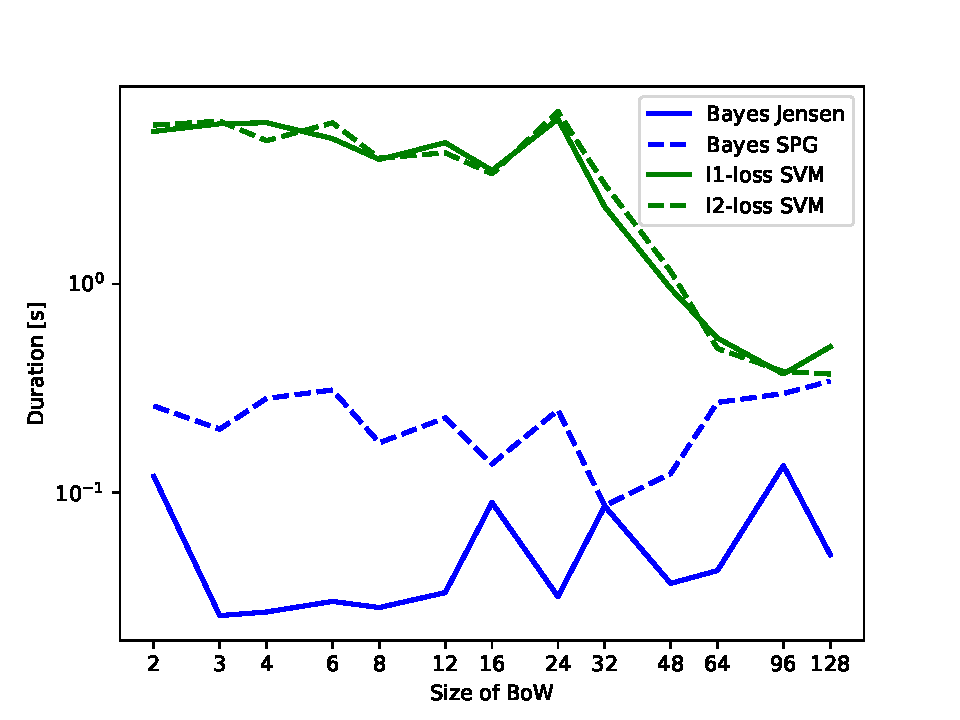
\includegraphics[width=\textwidth]{Figures/times.pdf}
    \end{minipage}%
    \begin{minipage}{.5\textwidth}
        \centering
        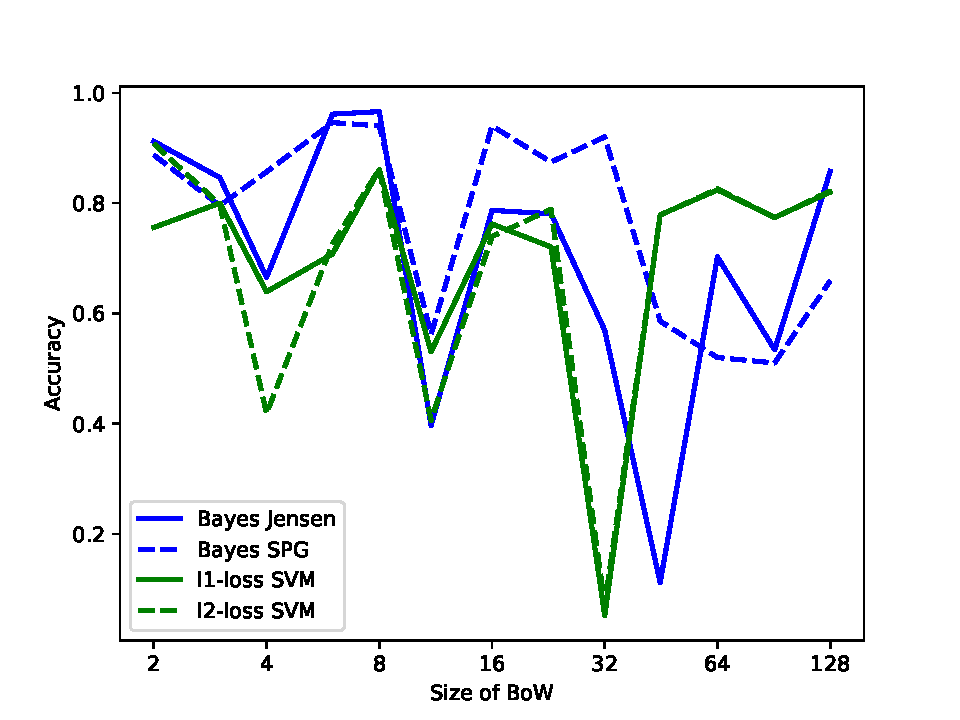
\includegraphics[width=\textwidth]{Figures/score.pdf}
    \end{minipage}
    \caption{The training duration and accuracy for different sizes of BoW.}
    \label{fig:results:graph}
\end{figure}

From the graphs \figref{fig:results:graph} we can observe that for the lower BoW sizes both versions of the Bayes classifier perform better in regards to accuracy and the duration of training. However, with the larger BoW sizes, both the $l1$-loss and the $l2$-loss regularized SVM performs similarly to the Bayes classifier.

\section{Conclusion and Acknowledgement}
The performance of the Bayesian model shows significant improvement, compared to the performance of the SVM. Further results will be presented at ICNAAM 2021.

This contribution has been completed thanks to the financial support provided to VSB-Technical University of Ostrava by the Czech Ministry of Education, Youth and Sports from the budget for conceptual development of science, research and innovations for the 2021 year.

\bibliographystyle{aipnum-cp}
\bibliography{DorCer_icnaam2020}

\end{document}
